\chapter{Representation of Environments}

\textbf{Author: Fabian Kleinrad} 

This chapter is going to concern itself with the critical intersection of physical and digital space. Fundamental for autonomous navigation to work are means for the algorithm to observe its surrounding. In order to accomplish a translation from physical space to a medium tailored towards information propagation, a SLAM algorithm, which is described in detail in chapter \ref{chapter:slam}, is being used. These following sections are going to explore the data, which is the output of the mapping phase and input into the path planning phase.

\section{Abstract Environments}

Abstraction being the process of reducing an Object to the information needed for further processing. In conjunction with autonomous navigation this principle is ubiquitous. Due to restriction in terms of computational space and time, a simplification of complex compounds is needed. Such a loss of information naturally happens when using equivalent hardware to process ones surroundings.\newline
In order for autonomous navigation to work it is necessary for the computer to know the existence and position of objects surrounding the to be navigated vessel. This information can be provided or in case of using a SLAM algorithm self-taught. SLAM reduces the environment to positions in a 2 or 3 dimensional space. The algorithm is then left with an assortment of positions relative to the starting point, which is represented by the coordinate origin. To make use of this information is imperative to know the position of the robot in this abstracted space.\newline
With this approach to let the of letting the algorithm perceive the environment it guarantees an efficient and cost effective computation. By reducing obstacles to only the properties needed to avoid them unnecessary complexity is being circumvented.      

\section{Representation in Autumn}
To be able to utilize the information provided, there need to be the capability of bundling data into a tried and tested format, that enables easy access and reliable accuracy.\newline
Autumn uses the occupancy grid and point cloud as means to represent the data acquired in the mapping stage. The occupancy grid serves its purpose in a 2 dimensional environment, where as on the contrary the point cloud is utilized in 3 dimensional use cases.

\subsection{Occupancy Grid}
An occupancy grid is used for a 2-dimensional representation of the environment. Hereby in case of an occupancy grid, a grid structure is being overlaid over the environment. Therefor it is possible to discretize the world into cells. Each cell contains information about the probability of being occupied. In this context the assumption is made, that cells can either one of the two states. Thus it allows for a simplification of algorithms needed to update such data structures, because with this assumption it allows for the use of binary random variables. Grid cells which are for certain occupied are represented by 1, which relates to the 100 percent probability of being occupied. Contrary free cells are described by a 0 percent probability of being occupied. Visually these features are displayed by coloring the cells black and white and every probability in between.\footcite{OccupancyGridMaps2020}

\begin{figure}[h]
	\centering
	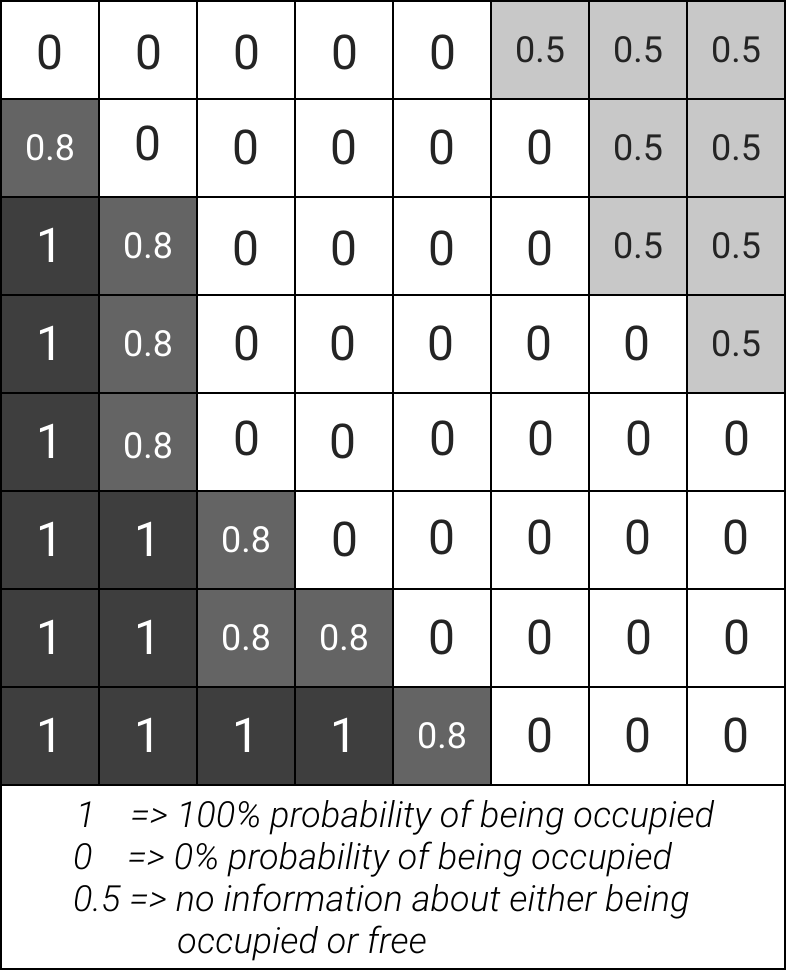
\includegraphics[width=0.5\linewidth]{img/OccupancyGridCells}
	\caption{Visual depiction of probability values in an occupancy grid map.}
	\label{fig:abstract_environments_occupancyCells}
\end{figure}

To add to the simplicity of the data structure and lower the time needed to update, two additional assumptions are made. The occupancy grid as well as many other assume a static world, which entails that occupied cells stay that way as well as their unoccupied equivalent. Secondly cells are viewed as individuals with know influence to their neighboring cells. This simplifies the calculations of probabilities, because of it the probability is the product of probability of single sensor readings.     

\subsection{Point Cloud}

\subsection{ROS Types}

\section{Abstracted Environments in Autumn}

\subsection{autumn$\_$pathfinding$\_$2D}

\subsection{autumn$\_$pathfinding}